%----------------------------------------------------------------------------
\chapter{Háttérismeretek}\section{A monitorozás alapjai}

Egy monitor feladata az, hogy futási időben egy rendszert megfigyeljen, elemezzen és egy adott követelmény alapján felismerje a rendszer helytelen viselkedését.
Ezt a helytelen viselkedést jelzi a rendszernek, de néhány esetben a rendszer működését is befolyásolhatja.
Ez egy kritikus rendszernél különösen fontos lehet hiszen, egy ilyen rendszernél elvárt, hogy folyamatosan biztonságosan tudjon működni.
Ezen kívül, a monitornak időmérésre is szüksége van, mert a követelmény tartalmazhat időziteseket is.
Az 1.1. ábra bemutatja a monitorozás koncepcióját.

\begin{figure}[!ht]
    \centering
    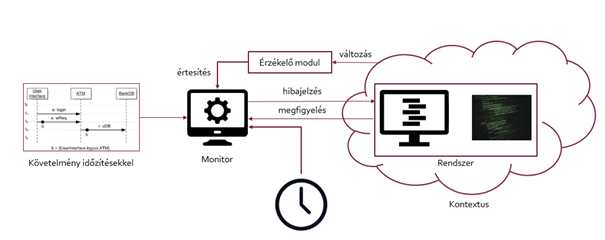
\includegraphics[width=150mm, keepaspectratio]{figures/1abra.png}
    \caption{Kontextusfüggő rendszerek monitorozása időzítési feltételekkel.}
\end{figure}

A scenario alapú monitorozás során a kommunikáció megfigyelésével szeretnénk felismerni a problémákat a rendszerünkben.
A rendszerben lévő objektumok közti interakciókat, üzeneteket fogja megfigyelni a monitor.
A követelményt scenario formájában adjuk meg az üzenet szekvenciák specifikálásához.
Szekvencia diagramok segítségével egyszerűen megadhatunk ilyeneket.
A diagramokat a későbbiekben olyan alakra kell majd hoznunk, hogy abból a monitor létrehozható legyen.

\clearpage\section{Időfüggő viselkedés specifikálására alkalmas formalizmusok áttekintése}
\subsection{MSC - Message Sequence Chart}

Az egyik legelterjedtebb scenario alapú modellezésre használt vizuális formalizmus a Message Sequence Charts (MSC).
A nyelv célja két, vagy több üzeneteket cserélő objektum között az interakciónak a leírása.
A Unified Modelling Language (UML) 2.0 szekvencia diagram leíró részét nagyban inspirálta ez a nyelv.
Az MSC főbb elemei:

\begin{itemize}
\item MSC head, lifeline és end
\item Objektum létrehozása
\item Üzenet csere
\item Függvényhívás és válasz
\item Timer-ek
\item Idő intervallumok
\item Összetett szerkezetek: alt, opt, parallel, loop (high-MSC)
\end{itemize}

Az összetett szerkezetek a high-MSC (h-MSC) nevű MSC kiterjesztésben találhatók.

Ezzel a nyelvvel már könnyedén lehet a scenarioban lévő üzeneteket specifikálni, és azokat a rendszer komponenseket, amelyek ezeket az üzeneteket egymásnak küldik.

Az UML és az MSC sokban hasonlítanak, de az alapelveik különbözőek.

MSC-ben a függőleges vonalak („life line”-ok) autonóm entitásokat képviselnek, míg a szekvencia diagramok esetén ezek egy objektumot reprezentálnak.
MSC esetén az entitásoknak nem szükséges ugyanazon a számítógépen lenniük.

MSC-ben egy átmenet egy aszinkron üzenetet reprezentál, amely két entitás között jött létre, míg az UML szekvencia diagram leíró nyelvében, egy átmenet egy függvényhívást jelent.

Az MSC-nek sajnos sok hiányossága is tapasztalható.
Hiányzik belőle az üzenetek típusossága.
Egy követelmény megfogalmazásakor fontos, hogy meg tudjuk mondani, melyek az elvárt üzenetek vagy, hogy melyek jelentenek hibát.
Az is nagy hiányosságnak számít,hogy az üzenetekre nem lehetséges megkötéseket megadni.
Ez egyben megnehezíti egy követelmény leírását is.

\subsection{MTL - Metric Temporal Logic}

A temporális logikák olyan formális rendszerek amelyekkel kijelentések igazságának logikai időbeli változását vizsgálhatjuk.
A kijelentések időbeli vizsgálásához temporális operátorokat használunk:
\begin{itemize}
    \item \textit{mindig}
    \item \textit{valamikor}
    \item \textit{mielőtt}
    \item \textit{addig, amíg}
    \item \textit{azelőtt, hogy}
    \item \textit{stb...}
\end{itemize}
A temporális logikákat két osztályba sorolhatjuk:
\begin{itemize}
    \item \textit{lineáris}
    \item \textit{elágazó}
\end{itemize}
A lineáris temporális logikáknál a model egy lefutását vizsgáljuk.
A logikai idő egy állapotsorozatnak tekintjük, ahol minden állapotnak egy rákövetkezője van.
Az elágazó temporális logikáknál viszont az összes lehetséges végrehajtást tekintjük.
A lineárissal ellentétben itt egy állapotnak több rákövetkezője is lehet és a logikai idő egy fa alakjában jelenik meg.

A \textit{Metric Temporal Logic} temporális operátorai a következők:
\begin{itemize}
    \item \textit{addig} (until)
    \item \textit{következő} (next)
    \item \textit{ettől} (since)
    \item \textit{előtt} (previous)
\end{itemize}
Az \textit{MTL} egy lineáris temporális logika, amely mind az átlapolt és kitalált idő absztrakciókat tekínti.
Logikai jelek tulajdonságait specifikálhatjuk vele az időben.

A szintaxisa a \textit{Linear Temporal Logic}-hoz hasonlít:
\begin{itemize}
    \item véges atomi kijelentések halmaza \textit{AP}
    \item $\neg$ és $\lor$ logikai operátorokat
    \item $U_I$ (\textit{Until}) temporális modális operátor, ahol egy \textit{I} egy nem negatív számokból álló intervallum
    \item $S_I$ (\textit{Since}) temporális modális operátor
\end{itemize}

A \textit{past-MTL} megfelel a teljes \textit{MTL}-nek az \textit{Until} operátor kivételével.
Hasonlóan, a \textit{future-MTL} a teljes \textit{MTL} a \textit{Since} operátor nélkül.

A cíkkekben változó, hogy az \textit{MTL}-t hogyan definiálják.
Az \textit{MTL} megegyezik az előbbi \textit{future-MTL}-el vagy a teljes szintaxissal van definiálva.

\subsection{MITL - Metric Interval Temporal Logic}

Az \textit{MITL} egy részhalmaza az \textit{MTL}-nek.
A definiciója megegyezik a \textit{MTL}-el azzal a megkötéssel, hogy az \textit{I} halmazok \textit{U}-ban és \textit{S}-ben nem egyedülállóak.
A halmazok határait természetes számok vagy végtelen határolják be.

\subsection{PSC – Property Sequence Chart}
%----------------------------------------------------------------------------
A Message Sequence Chart-nak nagyon sok hiányossága van.
Nem lehet vele megkötéseket definiálni vagy egy üzenetről eldönteni, hogy az egy elvárt vagy nem kívánt üzenet.
Ebből kifolyólag az MSC nem egy alkalmas nyelv arra, hogy az üzenet szekvenciáinkat részletesebben specifikálni tudjuk vele.

\begin{table}[ht]
    \centering % used for centering table
    \begin{tabular}{ |c|c|c| } % centered columns (4 columns)
    \hline
    \textbf{Tulajdonság} & \textbf{MSC} & \textbf{PSC} \\ [0.5ex] % inserts table
    %heading
    \hline % inserts single horizontal line
    \hline
    Nem kivánt üzenet & - & Fail message \\ % inserting body of the table
    \hline
    Elvárt üzenet & - & Required message \\
    \hline
    Sima üzenet & Default message & Regular message \\
    \hline
    Megkötött sorrendezés & - & Strict sequencing \\
    \hline
    Gyenge sorrendezés & Seq & Loose sequencing \\
    \hline
    Üzenet megkötések & - & Constraint \\
    \hline
    Alternatív lehetőségek & h-MSC & Alternative operator \\
    \hline
    Párhuzamos művelet & h-MSC & Parallel operator \\
    \hline
    Ciklus & h-MSC & Loop operator \\
    \hline %inserts single line
    \end{tabular}
    \label{table:nonlin} % is used to refer this table in the text
    \caption{Az MSC összehasonlítása a PSC-vel} % title of Table
\end{table}

A Property Sequence Chart[1] az MSC egy kiterjesztése.
Sok új elemet vezet be ami nincs az MSC-ben, melyek megtekinthetők a 2.1. táblázaton, mint az üzenet típusokat: sima üzenet (e), elvárt üzenet (r) és nem kívánt üzenet (f).
Így specifikálhatjuk, hogy mely üzenetek azok amik helyes viselkedésre utalnak és azok amelyek nem.
Az elvárt üzenetek azok az üzenetek amelyeknek feltétetlen meg kell történiük a rendszer működése során.
Egy sima üzenet nem jelent hibát a monitor szempontjából ha nem történik meg, viszont ha megjelenik, akkor a scenario-ban utána következő üzenetek ellenőrzésére kell áttérni.
Szigorú sorrendezésre is ad megoldást a PSC, ami azt jelenti, hogy megadhatjuk explicit az üzenetek sorrendjét a követelményünkben.
A PSC-ben egy üzenetre megkötést is rakhatunk.
Megadhatjuk, hogy melyek azok az üzenetek amik nem kívántak az üzenetünk előtt vagy után.
A különböző PSC tulajdonságok megtalálhatok a 2.1. ábrán.
A nyelv a következő tulajdonságokat támogatja:

\begin{itemize}
    \item \textit{Sima üzenet (e)}: egy üzenet a scenario-ban, amely ha nem történik meg az a monitor szempontjából nem jelent hibát.
    Viszont ha megjelenik, akkor a scenario-ban utána következő üzenetek ellenőrzésére kell áttérni.
    Egy előfeltételt reprezentál.
    \item \textit{Elvárt üzenet (r)}: egy üzenet amelynek elmaradása hibajelzéshez kell vezessen.
    \item \textit{Nem kívánt üzenet (f)}: amennyiben a monitor egy ilyen üzenetet detektál, akkor hibát jelez.
    \item \textit{Üzenet megkötés (constraint)}: Egy üzenetre lehet megkötést is helyezni.
    Egy megkötés több üzenetet tartalmazhat.
    Két fajta megkötést definiál a nyelv: múlt- és jövőbéli.
    A múltbéli üzenet megkötés esetén, az üzenetünk megtörténte előtt, a megkötésben szereplő üzenetek egyike se történhet meg.
    Jövőbéli megkötés esetén, pedig az üzenetünk megtörténte után nem történhetnek meg a megkötésben szereplő üzenetek.
    \item \textit{Megkötött sorrendezés (strict ordering)}: A PSC az üzenet lefutási sorrendjének a specifikálására is lehetőséget ad.
    Egy „a” üzenet megtörténte után, egy adott „b” üzenetnek kell bekövetkeznie.
    Ha „b” üzenet helyet egy másik üzenet követi az „a” üzenetet, akkor a monitor hibát jelez.
\end{itemize}

A nyelv támogat összetett szerkezeteket is:

\begin{itemize}
    \item \textit{Alt operátor}: az alt operátorral alternatív üzenet szekvenciákat lehet definiálni.
    \item \textit{Par operátor}: a par operátorral meghatározható az üzenet szekvenciák párhuzamos futása.
    \item \textit{Loop operátor}: a loop operátorral megadhatjuk, hogy egy üzenet szekvencia többször is lefuthat egymás után.
\end{itemize}

Egy üzeneten egyszerre megkötés és sorrendezés is lehet.
Az üzenetek típusát az átmenetén lévő karakterrel jelöljük.
Az „e” karakter jelzi, hogy az üzenet sima, az „r” karakter az elvárt üzenetet jelenti, az „f” pedig a nem kívánt üzenetet.
Azt meg kell jegyezni, hogy nem kívánt üzenetekre nem lehet jövőbéli megkötéseket rakni.
Ezen kívül, ha egy üzeneten megkötött sorrendezést alkalmazunk, akkor nem lehet rajta múltbéli megkötés.

A megkötéseket egy ponttal jelöljük, amit az átmeneten helyezünk el.
Ha a pont az átmenet elején van (a feladóhoz közel), akkor az múltbéli megkötést jelöl.
Ha pedig a végén helyezkedik el, akkor a jövőbéli megkötést jelöli.
A megkötésben lévő üzeneteket egy lista formájába lehet megadni ’{’ ’}’ jelek közt, a következő módon: <megkötés neve> = {C1.I1.Cj, ..., Ck.In.Ct}, ahol az üzenetek vesszővel elválasztva, „Feladó.Üzenet.Címzett” formában szerepelnek.
A specifikált megkötés nevét pedig az átmeneten lévő pont alá írjuk.

Az üzenetek megkötött sorrendezésének jelölésénél az objektum „life line” vonalát az érintett átmenetek közt folytonossá változtatjuk

\begin{figure}[!ht]
    \centering
    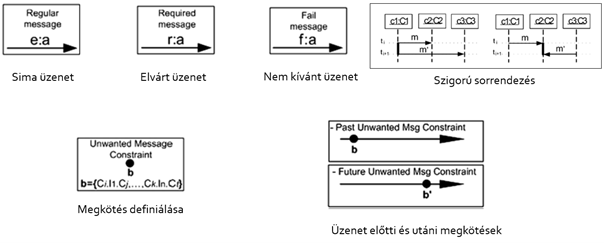
\includegraphics[width=150mm, keepaspectratio]{figures/2abra.png}
    \caption{A PSC különböző elemei[1].}
\end{figure}

Az üzeneteket a következő formában adjuk meg: \textit{Feladó.Üzenet.Címzett}.

\begin{figure}[!ht]
    \centering
    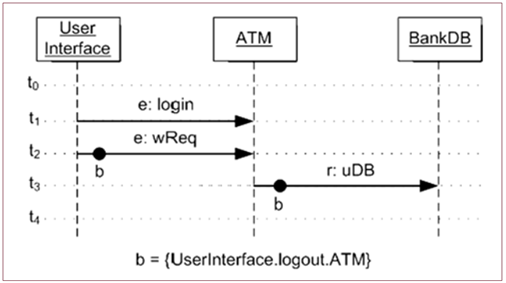
\includegraphics[width=130mm, keepaspectratio]{figures/3abra.png}
    \caption{PSC diagram egy ATM rendszer működésének ellenőrzésére[1].}
\end{figure}
A 2.2. ábrán láthatunk egy példát arra, hogy egy követelményt hogyan lehet definiálni.
Ez a PSC diagram egy ATM rendszer működését figyeli.
Először a felhasználó egy \textit{login} üzenettel bejelentkezik az ATM-be majd egy \textit{wReq} üzenettel egy lekérdezést hajt végre.
Ezen az üzeneten van egy megkötés, az üzenet előtt nem történthet kijelentkezés, \textit{logout}.
Az ATM ezután, ha nem történt \textit{logout} egy elvárt üzenetet küld a Bank adatbázisába.

A scenario-ink specifikálására most már rendelkezésünkre áll egy grafikus nyelv.
A következőkben az lesz a feladatunk, hogy ezeket a diagramokat úgy transzformáljunk, hogy monitor kódot lehessen belőlük készíteni.


%----------------------------------------------------------------------------
\clearpage\section{A TPSC bemutatása}
%----------------------------------------------------------------------------
A TPSC[2] a PSC-nek egy kiterjesztése.
A PSC üzenetekre időzítési feltételeket specifikálhatunk.

\begin{figure}[!ht]
    \centering
    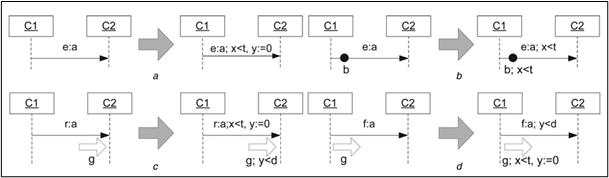
\includegraphics[width=150mm, keepaspectratio]{figures/4abra.png}
    \caption{PSC kiterjesztése időzítési feltételekkel[2].}
\end{figure}

A TPSC óraváltozókat (x, y) használ az időzítéshez.
Ezekre meg lehet adni feltételeket, valamint az óraváltozót lehet nullázni.
A nullázással adott eseménytől (pl. üzenet vételétől) kezdve indul az időzítés, majd rákövetkező események időbeliségét ez alapján lehet ellenőrizni.

A 3.1. ábrán látható, hogy például az \textit{e: a} sima üzenet \textit{e: a; x < t, y := 0} üzenetre bővül.
Elvárjuk, hogy az \textit{a} üzenet \textit{t} idő előtt történjen meg és egy \textit{y} óraváltozót nullázunk.
Az \textit{e: a} üzenet egy sima üzenet, szóval ha nem történik meg a specifikált idő intervallumban az nem jelent hibát.
Viszont \textit{r: a} üzenetnél már elvárt, hogy \textit{t} időn belül megtörténjen. \textit{f: a} üzenet esetében viszont akkor jelez hibát a monitor, ha üzenet megtörtént \textit{t} időn belül.

Egy megkötésre is meg lehet adni időzítési feltételt.
Így megadhatjuk, hogy mennyi ideig nem szabad jönnie a megkötésben szereplő nem kivánt üzenetek egyikének.
Ha a feltételben megadott idő után történik akkor az nem jelent hibát a monitor szempontjából.

% !TeX spellcheck = hu_HU
% !TeX encoding = UTF-8
% !TeX program = xelatex
%----------------------------------------------------------------------------
\clearpage\section{TPSC szcenário alapú automata konstrukció}
%----------------------------------------------------------------------------

A monitorozás alapja, hogy TPSC scenario-kból időzített automatákat (Timed Automata) tudjunk készíteni.
Egy TA állapotokból, elfogadó állapotokból, feltételekből, akciókból és bemenetekkel címkézett állapotátmenetekből áll.
Akkor fogad el egy bemenet sorozatot, ha ennek során elérünk az automata végállapotába.
Ha elfogadó állapotot érünk el, akkor az a monitor szempontjából hibát jelent.
Az alapelv az az, hogy minden TPSC elemhez tartozik egy minta automata (pattern) ami leírja a szemantikáját.
Például a 4.1. és 4.2. ábrákon láthatóak a különböző PSC üzenetekhez tartozó minták.

\begin{figure}[!ht]
    \centering
    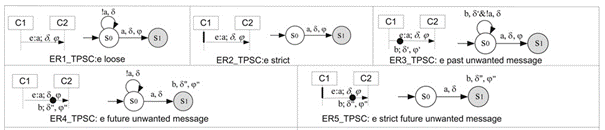
\includegraphics[width=150mm, keepaspectratio]{figures/5abra.png}
    \caption{Sima üzenetekhez tartozó minták[2].}
\end{figure}

\begin{figure}[!ht]
    \centering
    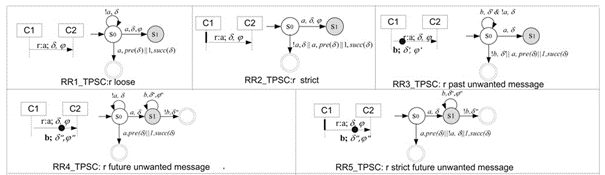
\includegraphics[width=150mm, keepaspectratio]{figures/6abra.png}
    \caption{Elvárt üzenetekhez tartozó minták[2].}
\end{figure}

A minta automatánkban található szürke állapotok reprezentálják a végállapotokat.
A megkötéseket az automatáknál egy átmenettel definiáljuk ami a nem kívánt üzenetek negáltjainak az ÉS kapcsolata.
Például az 4.1. ábrán lévő 3. automata mintán látható „b, $\delta ’\&!a, \delta$” címkéjű hurokélen, a „b” címke minden olyan üzenetnek felel meg, amelyek nincsenek a nem kivánt üzenetek halmazában.
A címke teljes jelentése az, hogy ha $\delta$’ időn belül nem jött nem kivánt üzenet és $\delta$ időn belül nem az „a” üzenet jött akkor maradjunk az s0 állapotban.
Ezekből az automata részekből lesznek meghatározott illesztési szabályokkal a scenario-hoz tartozó teljes időzített automaták.
Ennek az az alapelve, hogy a scenario-n végig menve az előző minta végállapotát a következő minta kezdőállapotával kell egyesíteni.
Ezt a folyamatot mutatják be a 4.3., 4.4. és 4.5. ábrák.

\begin{figure}[!ht]
    \centering
    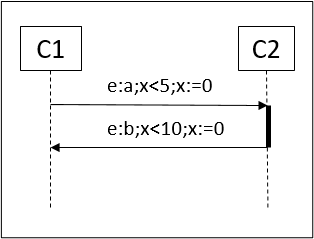
\includegraphics[width=60mm, keepaspectratio]{figures/7abra.png}
    \caption{TPSC részlet.}
\end{figure}

\begin{figure}[!ht]
    \centering
    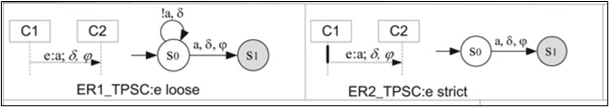
\includegraphics[width=150mm, keepaspectratio]{figures/8abra.png}
    \caption{Alkalmazott automata minták.}
\end{figure}

\begin{figure}[!ht]
    \centering
    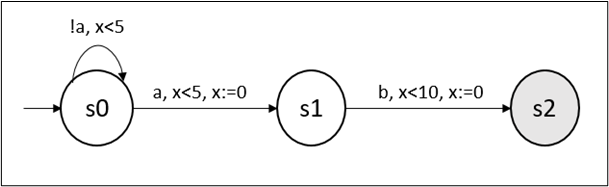
\includegraphics[width=130mm, keepaspectratio]{figures/9abra.png}
    \caption{Az összeállított automata.}
\end{figure}

A monitor szempontjából az automata akkor jelez hibás működést ha elfogadó állapotba kerül.
Ilyenkor a követelmény már nem teljesíthető.
Ha az automata egy sima állapotban van, akkor az helyes működést jelent viszont a követelmény még ekkor sem teljesült.
A követelmény akkor teljesül amikor az automata a végső (FINAL) állapotba kerül és nem érkezik további amely elmozditaná őt onnan.